%%%%%%%%%%%%%%%%%%%%%%%%%%%%%%%%%%%%%
%%%%% PHYS305 Assignment 3
%%%%% Zachary Martin
%%%%% 6 February 2019
%%%%%%%%%%%%%%%%%%%%%%%%%%%%%%%%%%%%%

\documentclass[aps,prl,twocolumn,superscriptaddress]{revtex4-1}

\usepackage{graphicx}  % this is the up-to-date package for all figures
\graphicspath{{pictures/}} 	% Set Graphics Path
\usepackage{siunitx} % Scientific Notation and Units
\usepackage{amsmath, amssymb, gensymb, mathtools, bm, bigints} 	% Mathematical Tools
\usepackage{verbatim}  % for the comment environment
\usepackage{color}
% \usepackage{arydshln} % Dashed lines in table

% For inserting code snippets
\usepackage{listings}
\usepackage{xcolor}
\lstset { %
    language=C++,
    backgroundcolor=\color{black!5}, % set backgroundcolor
    basicstyle=\footnotesize,% basic font setting
}

% Shortcut Commands
\newcommand{\paren}[1]{\left( #1 \right)} 	% Parentheses for complicated expressions
\newcommand{\bparen}[1]{\left[ #1 \right]}	% Bracket parentheses for complicated expressions
\newcommand{\cmod}[1]{\left| #1 \right|}	% Mod or Absolute value

\bibliographystyle{apsrev}

% these are some custom control of the page size and margins
% \topmargin= 0.2in  % these 1st two may be needed for some computers
\textheight=9in
\textwidth=6.5in
% these next two lines give us centered text
\oddsidemargin=0cm
\evensidemargin=0cm

\begin{document}

% Title Contents
\title{PHYS 305 Assignment 3: Numerical Integration and Analysis of Chirp Functions.}
\author{Zachary Martin}
\affiliation{University of Hawaii at Manoa}
\date{6 February 2019}

\begin{abstract}
In this assignment, we examine the techniques used to integrate functions using numerical methods in C++. Specifically, we look at the Trapezoidal rule and Simpson's rule for approximating integrals. Their rate of convergence is examined using a known integrable function. Then we then apply these techniques to a damped chirp function and analyze the results obtained from there. We find how the sum over the chirp function changes as a function of time and use this to find that the energy per unit area of the chirp is $E/A = \SI{3.48237}{\joule\per\m\squared}$. We also find that the intensity of the chirp is $I = \SI{0.435}{\watt\per\m\squared}$ or $I = \SI{116.4}{\decibel}~$.
\end{abstract}

\maketitle

\section{Introduction and Overview}
While we encounter many mathematical problems in physics that are solvable, a countless number of problems are not solvable exactly, that is, the solutions have no analytic form. It is therefore important to learn numerical techniques and how to employ them efficiently using computational methods.

Chirp functions are a fairly simple example of non-integrable functions. And yet, the integral of a chirp function is physically useful in understanding acoustics. We need this to find the energy and intensity in an acoustic wave pulse.
 
\section{Description of Computational Problem}
To compute integrals, we must use approximation methods by summing up small areas under the curve made by the integrand. There are many ways to do this, but some are more accurate than others. Two useful methods are the Trapezoidal rule and Simpson's rule. These are different summation series assuming certain shapes made by the area under the curve within a small interval using values from the function of interest (the integrand).   Thus, we will need to be able to define a function which follows these sums. In the process, we can look at how changing the number of intervals between two fixed limits of integration affects the value of the integral or sum of the series.

We then apply this to a chirp function and examine how the value changes with time. This will then tell us about the energy density of the wave pulse described by the chirp function. The details of these calculations are discussed in the next section.

\section{Relevant Equations}
The Trapezoidal rule takes an interval and assumes the shape of the area under the curve to be a trapezoid via connecting the two points at the endpoints of the interval in a straight line \cite{trap}. Then the area of that trapezoid is just
\begin{equation}
\int_{x_1}^{x_2} f(x) dx = \frac{1}{2} \paren{x_2 - x_1} \paren{f(x_1) + f(x_2)} ~. \label{eqn:trap}
\end{equation}
If we split the interval $[x_1, x_2]$ into much smaller intervals, we can sum over all the corresponding areas to get a more accurate integral value. We do this with the following function:

\begin{lstlisting}
double trapez (int no, double min, double max)
{			
   double interval, sum=0., x;		 
   interval = ((max-min) / (no-1));
   sum += 0.5 * f(min) * interval;
   for (int n=2; n<no; n++)
   {
      x = min + interval * (n-1);      
      sum += f(x)*interval;
   }
   sum += 0.5 *f(max) * interval;
   return (sum);
\end{lstlisting}
The other approximation is using Simpson's rule. This method differs from the trapezoidal rule in that instead of connecting the two points in a straight line, they are connected using a quadratic curve \cite{simp}. To sum over these areas, we require that an odd number of intervals, and then the areas are just
\begin{equation}
\int_{x_1}^{x_1 + 2 h} f(x) dx = \frac{1}{3} h \paren{f_1 + 4 f_2 + f_3} ~. \label{eqn:simp} 
\end{equation}
Here, $h$ is the step size. Then again, we can sum over many areas of this type using
\begin{lstlisting}
double simpson (int no, double min, double max)
{  				 
   double interval, sum=0., x;
   interval = ((max -min) /(no-1));
   for (int n=2; n<no; n+=2)
   {
       x = min + interval * (n-1);
       sum += 4 * f(x);
   }
   for (int n=3; n<no; n+=2)
   {
      x = min + interval * (n-1);
      sum += 2 * f(x);
   }   
   sum +=  f(min) + f(max);
   sum *= interval/3.;
   return (sum);
\end{lstlisting}
Now we can apply these to any function that we define. The function in particular that we are interested in is the chirp function, which looks like
\begin{equation}
f(t) = \cos t^3	~.	\label{eqn:chirp}
\end{equation}
More specifically, we will examine the chirp function with an exponential decay or dampening factor. So we have
\begin{equation}
p(t) = 20*\cos t^3 \exp \paren{-\paren{\frac{t}{4}}^8} ~, \label{eqn:chirpe}
\end{equation} 
The function represents pressure in a sound wave, so we have chosen an amplitude of $\SI{20}{\pascal}~$. This is seen more clearly in Figure \ref{gr:chirp}. The intensity is related to the pressure by \cite{inten}
\begin{equation}
I = \frac{dP}{dA} = \frac{d^2 E}{dA dt} = \frac{p(t)^2}{\rho c} ~, \label{eqn:inten}
\end{equation}
where $\rho = \SI{1.2}{\kg\per\m\cubed}$ is the density of air at sea level, and $c = \SI{340}{\m\per\s}$ is the speed of sound in air at sea level. Through the second half of Equation \ref{eqn:inten}, we can find the energy per unit volume of the chirp by taking
\begin{equation}
\frac{dE}{dA} = \frac{E}{A} = \bigintsss_{t_1}^{t_2} \frac{\paren{\cos \paren{(\omega t)^3} \exp \paren{-\paren{\frac{t}{4}}^8}}^2}{\rho c} dt \label{eqn:fchirp}
\end{equation}
We can then find the intensity by examining the rate of change of the energy per unit volume with time. Another way we can express intensity is using decibels. To obtain the decibel value of intensity, we use \cite{Laulima}
\begin{equation}
\SI{1}{\decibel} = 10 \log \frac{I}{I_\text{ref}} ~, \label{eqn:db}
\end{equation}
where $I_\text{ref} = \SI{1e-12}{\watt\per\meter\squared}~$.

\section{Results and Graphs}

\begin{figure}[htbp]
  	\begin{center}
 		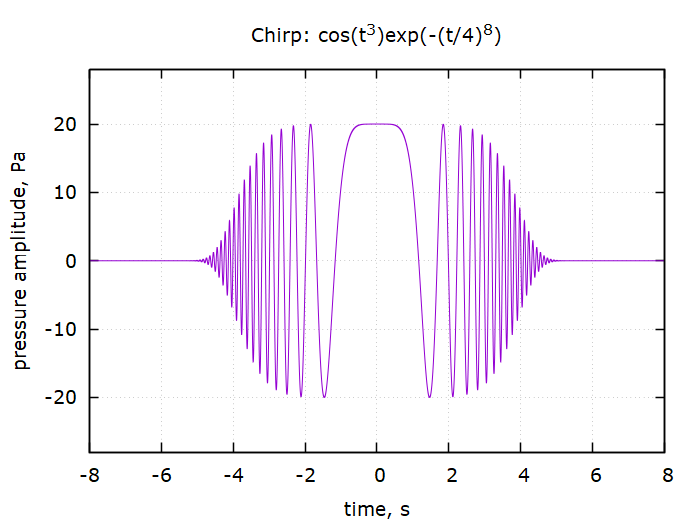
\includegraphics[scale=0.3]{chirp.png} 
  		\caption{The chirp function. Notice how the function exhibits sharp changes in frequency. This behavior causes the function to be non-integrable.}
  		\label{gr:chirp}
 	\end{center}
\end{figure}

\begin{figure}[htbp]
  	\begin{center}
  		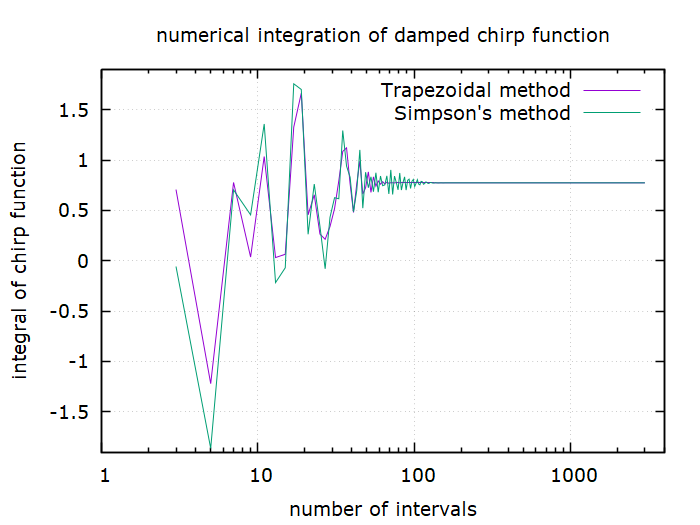
\includegraphics[scale=0.3]{t3.png} 
 		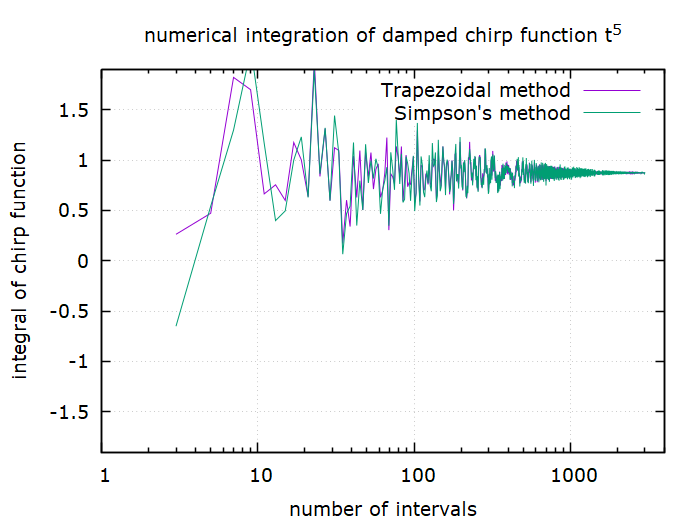
\includegraphics[scale=0.3]{t5.png} 
  		\caption{Integral values of the chirp functions for leading terms $\cos t^3$ (top) and $\cos t^5$ (bottom) using the Trapezoidal and Simpson's rules as a function of interval number ($dt$ size).}
  		\label{gr:int}
 	\end{center}
\end{figure}

\begin{figure}[htbp]
  	\begin{center}
 		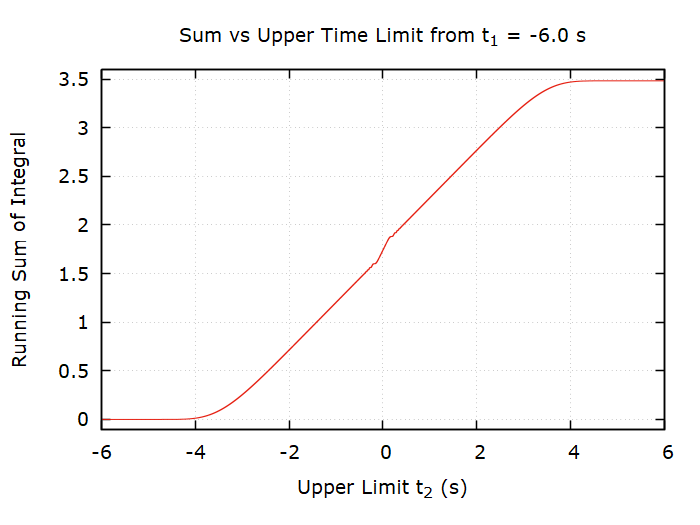
\includegraphics[scale=0.3]{sum.png} 
  		\caption{The cumulative sum or the integral value of Equation \ref{eqn:fchirp} as a function of time. The lower limit is fixed at $t_1 = \SI{-6.0}{\s}~$. Notice that the graph exhibits a linear behavior from $\SI{-4.0}{\s}$ to $\SI{4.0}{\s}$ until plateauing to the final cumulative sum (sum doesn't increase before and after the chirp).}
  		\label{gr:sum}
 	\end{center}
\end{figure}

\section{Discussion and Analysis}
From Figure \ref{gr:int}, we can see that a smaller degree results in a faster convergence. Before convergence, both methods give alternating values, and this is due to the positive and negative values of the chirp function, thus positive and negative integral values. We can also see that although the Simpson's rule can often be a better approximation for integrating, it converges more slowly to the integral value than the Trapezoidal rule. Nonetheless, there is still a clear agreement from the two methods once beyond a certain number of intervals.  We can be certain then when we integrate the new chirp function to find $E/A$ that we should find a stable value if we can choose a big enough number of intervals. Through trial and error, we find that the number of intervals to get a stable value for Equation \ref{eqn:fchirp} is around $N = 90221$, or a $dt$ size of $dt = \SI{1.33e-4}{\s}~$.

We can interpret from Figure \ref{gr:sum} that the energy per unit area increases almost linearly during the pulse. This implies from Equation \ref{eqn:inten} then that the power of the pulse is nearly constant. We can also see that the total energy per unit area of the chirp is $E/A = \SI{3.48237}{\joule\per\m\squared}$.

From Equation \ref{eqn:inten}, we can use the slope in Figure \ref{gr:sum} from $\SI{-4.0}{\s}$ to $\SI{4.0}{\s}$ to get an approximation for $I$. We get that $I = \SI{0.435}{\watt\per\m\squared}$. Then using Equation \ref{eqn:db}, we find that this corresponds to an intensity of $I = \SI{116.4}{\decibel}~$, about the same intensity as a rock concert \cite{Laulima}.

\section{Conclusions}
We were able to explore the computational methods of numerical integration and apply it to the unintegrable chirp function. Knowing the solvable acoustic relations that the chirp function described, we were able to find that the pulse produced a total energy per unit area of $E/A = \SI{3.48237}{\joule\per\m\squared}$ and an acoustic intensity of $I = \SI{116.4}{\watt\per\m\squared}$ or $I = \SI{116.4}{\decibel}~$. These techniques can be used to numerically solve many more types of integrals we may encounter in physics, which opens up opportunity to explore various complex systems. 

\section*{Acknowledgments}
\setlength{\parindent}{0cm}

\bibliographystyle{aipauth4-1}
\bibliography{bib3}



\end{document}